% !TeX spellcheck = en_US
\documentclass[11pt, fleqn, titlepage]{article}
%\usepackage{siunitx}
\usepackage{texfiles/SpeedyGonzales}
\usepackage{texfiles/MediocreMike}
\newcommand{\so}[2]{{#1}\mathrm{e}{#2}}
% \geometry{top=1cm}
\usepackage{hyperref}
\usepackage{amsmath}
\usepackage{ragged2e}
\usepackage{booktabs}
\hypersetup{
	colorlinks=true,
	linkcolor=blue,
	filecolor=magenta,      
	urlcolor=cyan,
}
\usepackage{subfig}
\usepackage{graphicx}
\title{Human arm trajectories in obstacle avoidance}
\author{Oskar Eiler Wiese Christensen s183917 \\ Anders Henriksen s183904 \\ \\ 02445 Project in Statistical Evaluation of Artificial Evaluation}
\date{\today \vspace{2.5cm} \section*{\small Summary} 
%\textit{The summary should contain a summary of the problem that  you are working with, which results you got, as well as main conclusions. \\ Don’t get into technical details. The summary should not be very long} \\ 
%Purpose and importance of the research
%What has been done
%What has been found
%Implications of the research
\justify{\footnotesize  Security and access authorization plays a big role in modern society. Improvement of these systems could be accomplished by using movement curves to identify the person and give access only to those with authority. The purpose of this paper is to investigate if it is possible to identify people based on movement curves by using two machine learning models, K-nearest neighbors and a binary decision tree, as well as to test if experiment has a significant effect on curve. The results show that it is to some extent possible to predict person from curve and that KNN is most effective at this task. Meanwhile, experiment has a significant effect on curve. This implies that movement curves might be useful for classifying people if using more complicated machine learning models. Meanwhile, performing different actions lead to different curves, which has positive implications for the possibility of movement-based surveillance.}}

\pagestyle{plain}
\fancyhf{}
\rfoot{Page \thepage{} of \pageref{LastPage}}

\graphicspath{{Billeder/}}

\begin{document}

\maketitle
%\thispagestyle{fancy}
%\tableofcontents

\section{Introduction}
%\textit{Briefly introduce the background and setting of the problem, as well as the aim of the report. Furthermore, you could give a very short description of the analysis that will be applied.} \\
Security plays a larger role in life every year, whether used for personal security or for the governmental spying on billions. Throughout the years, sercurity has taken many forms like facial and voice recognition, but movement recognition, if it proves successful, could turn out to be an effective way of finding perpetrators of crimes or locking people into their own homes. For this to truly be effective, it should be possible to classify people based on their movements and maybe even recognize actions based on the motion curve.

This is exactly what is wished to be accomplished in this paper; Classify the person performing the action based on the given motion curve using decision trees and K-nearest neighbors, and analyzing whether the type of obstacle has an influence on the resulting curve by the use of ANOVA. For this, the focus has been specifically on the arm movement dataset from \textbf{Grimme et al. 2014} \cite{armdata}. The hypothesis prior to the carrying out of the experiment was that it should be possible to classify the person based on the curve, since people can move in substantially different ways. It is also expected that experiment should play a significant role on the resulting curve, since a much larger obstacle should make people lift their arms much more dracstially.

\section{Data}
%\textit{Describe of the data you are analyzing. What kinds of data do you have, how were they collected (if applicable)? \\ Include a few good plots to highlight important features in data. You can put additional plots in the appendix.}
%*\textbf{Description of data:}
Ten different test subjects performed obstacle avoidance tasks on a table by relocation of a cylindrical object from position A to position B. Different experiments, with varying heights of the obstacle, were executed, and the test subjects were furthermore asked to avoid the obstacle by lifting the cylindrical object at hand. The movements were recorded with VZ 4000. The trajectories of markers were recorded using a sampling rate of 110 Hz. The starting position projected to the table is considered the origin in a three dimensional space. Fifteen different obstacle avoidance experiments were conducted, with one experiment for every combination of the blocks S,M, or T with the given measure $ d \in \{15, 22.5,  30, 37.5, 45\} $ as well as a control experiment with no obstacle. Each person repeated each of the sixteen different experiments ten times. The full data has a total size of $ m_f = 174,160 $. \cite{armdata}
\begin{figure}[H]
	\centering
	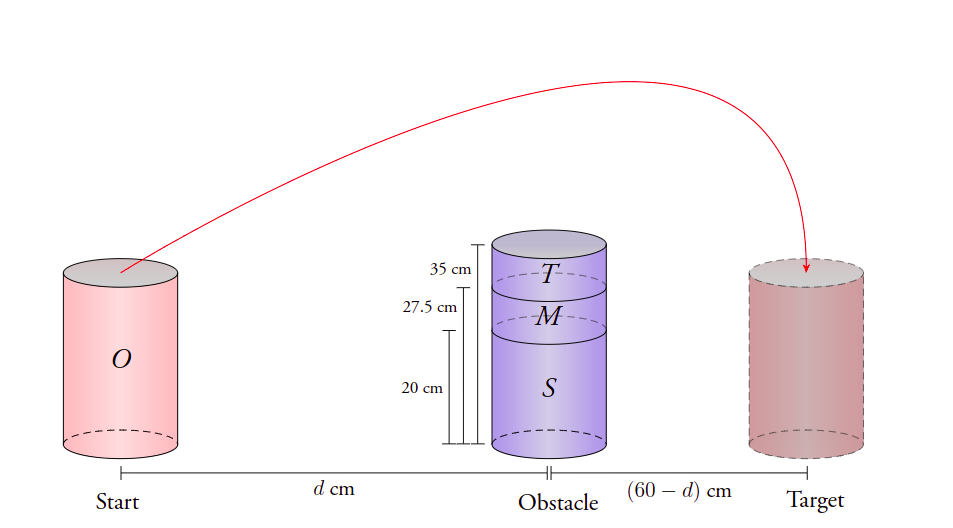
\includegraphics[width=0.5\linewidth]{billeder/exp_pic.png}
	\caption{An illustration of the obstacle avoidance setup. Test subjects have to move the cylinder from start to the finnish position "target", while avoiding the blue obstacle.}
	\label{fig:exppic}
\end{figure}
The data itself consists of recorded trajectory movements, by measured $ x,y,z $-coordinates in a three dimensional space. An illustration of the coordinates are given in \ref{fig:rplot}. Here the variables S, M and T vary in the different experiments. An example of ten different arm-trajectory paths of a test subject repeating the same experiment is shown in the figure \ref{fig:rplot}.

\begin{figure}[H]
	\centering
	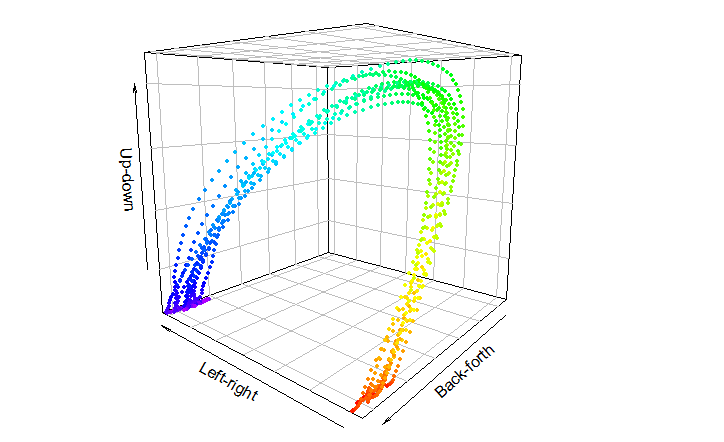
\includegraphics[scale=0.6]{billeder/Rplot.png}
	\caption{An illustration of test subject 1's arm trajectories in experiment one. Each of the lines in the plot illustrate a repetition in the experiment. }
	\label{fig:rplot}
\end{figure}

In figure \ref{fig:rplot} the path of the arm trajectories indicates that just in one persons repetition of the same experiment there is a lot of variation. Below is shown a boxplots of the variation in the Z-dimension of all the test subjects.

\begin{figure}[H]
	\centering
	\includegraphics[width=0.7\linewidth]{billeder/boxplot_z.pdf}
	\caption{Boxplots of the variation in the Z-dimension of the arm trajectories for all test subjects}
	\label{fig:boxplotz}
\end{figure}

Figure \ref{fig:boxplotz} presents a notable variation in the Z-dimension which suggests that it may be possible to distinguish each test subjects trajectory arm movements. In \ref{fig:boxplotz}, the variation is greater for $ z \in [13,85] $ than at the beginning and end of the movement curve, which makes sense since each subject moves the cylindrical object from the same start position to the same end position.
\\\\
A principle component analysis is done in order to investigate the dimensionality and variation of the data. The analysis yields a hundred principle components, whereas a lot of the variation is explained by the first couple of principle components as illustrated in \ref{fig:varexp}.

\begin{figure}[H]
	\centering
	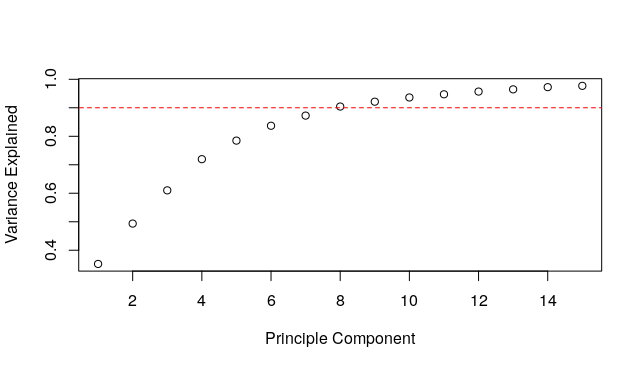
\includegraphics[width=0.7\linewidth]{billeder/varexp.png}
	\caption{A variance explained graph. The graph shows the variance explained cumulatively by the number of principle components. The red line in the plot indicates a threshold at 90\% explained variance.}
	\label{fig:varexp}
\end{figure}

In order to explain 90 \% of the variation of the data, the first eight principle components are needed, which also can be noted from figure \ref{fig:varexp}. By having a great proportion of the variance explained by relatively few principle components it seems possible to construct a classifier in order to determine a person from his/her trajectory paths.
\\
To get a visual grasp of the original data points projected onto the space of the principle components, a scatter plot of the transformed data in the principle component space is plotted, as seen below.

\begin{figure}[H]
	\centering
	\subfloat[label 1]{{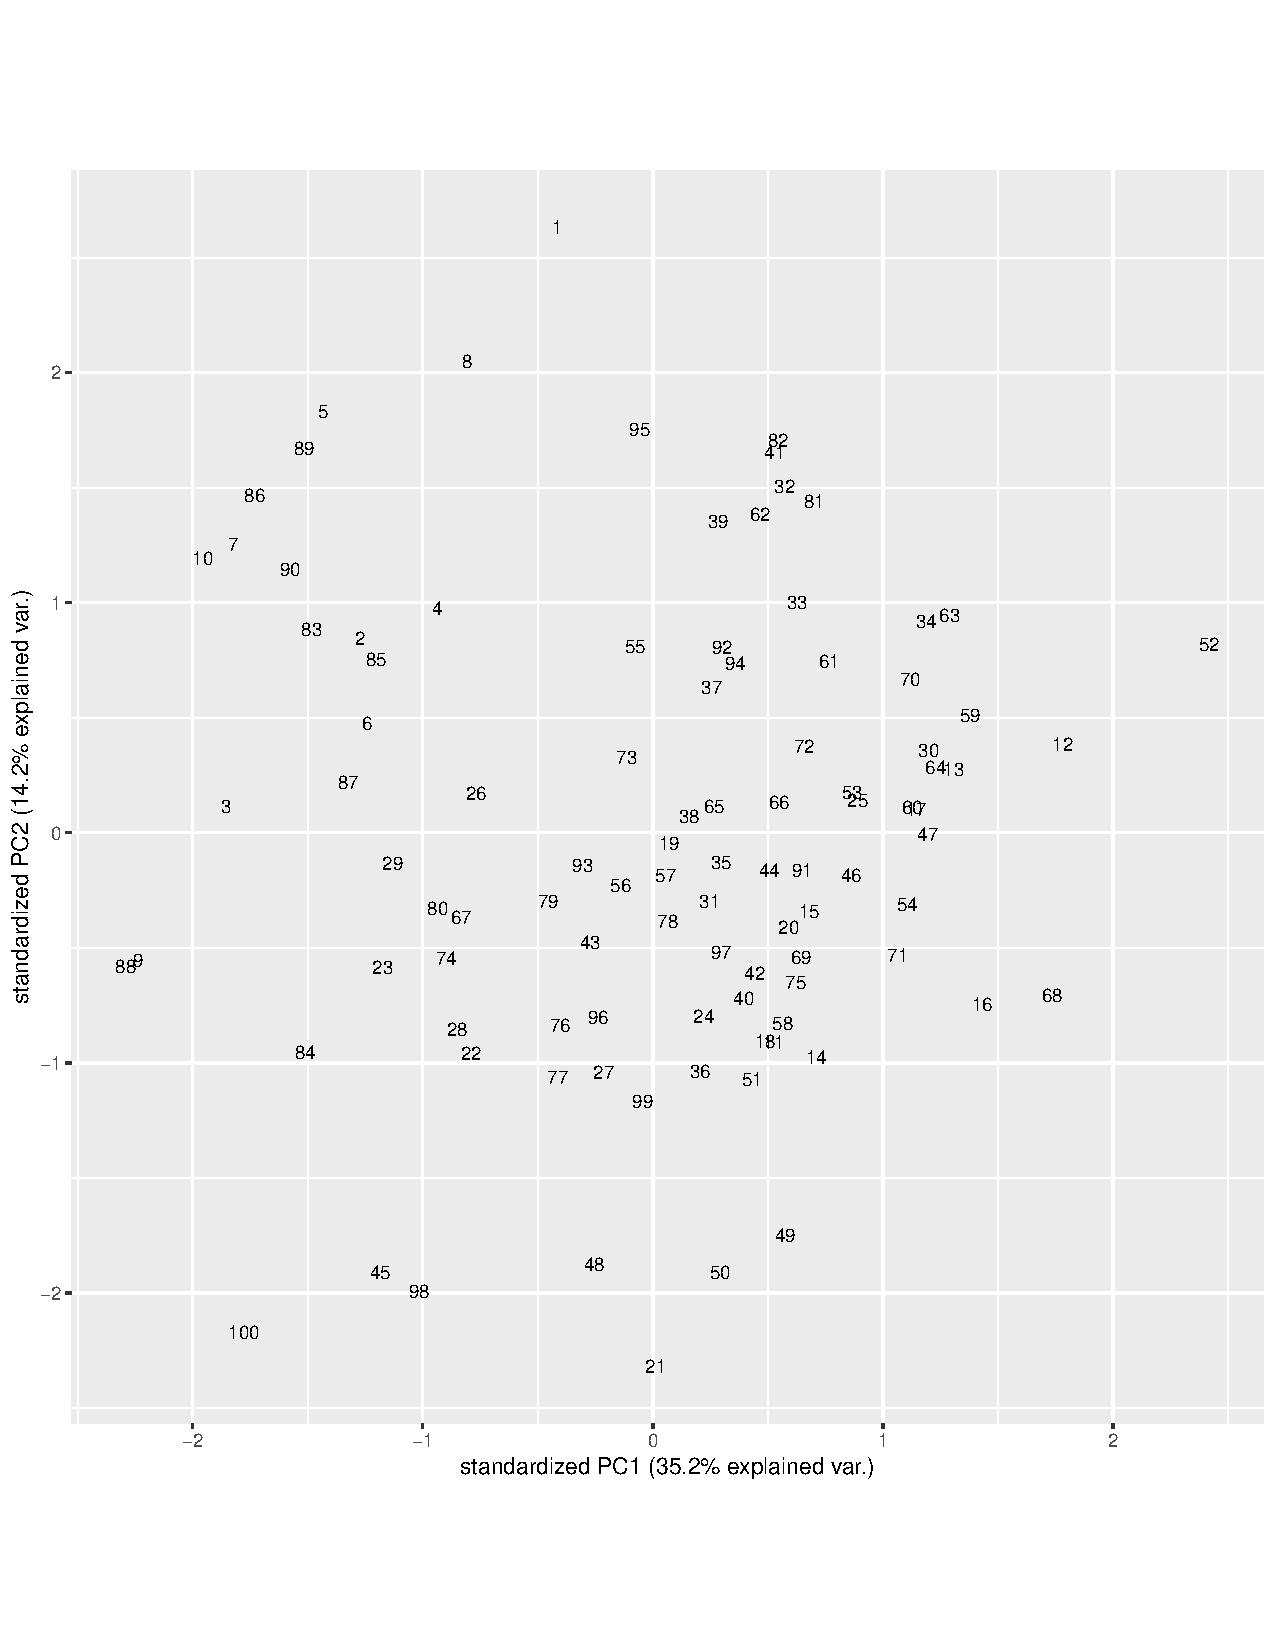
\includegraphics[width=5cm]{billeder/pca1.pdf} }}%
	\qquad
	\subfloat[label 2]{{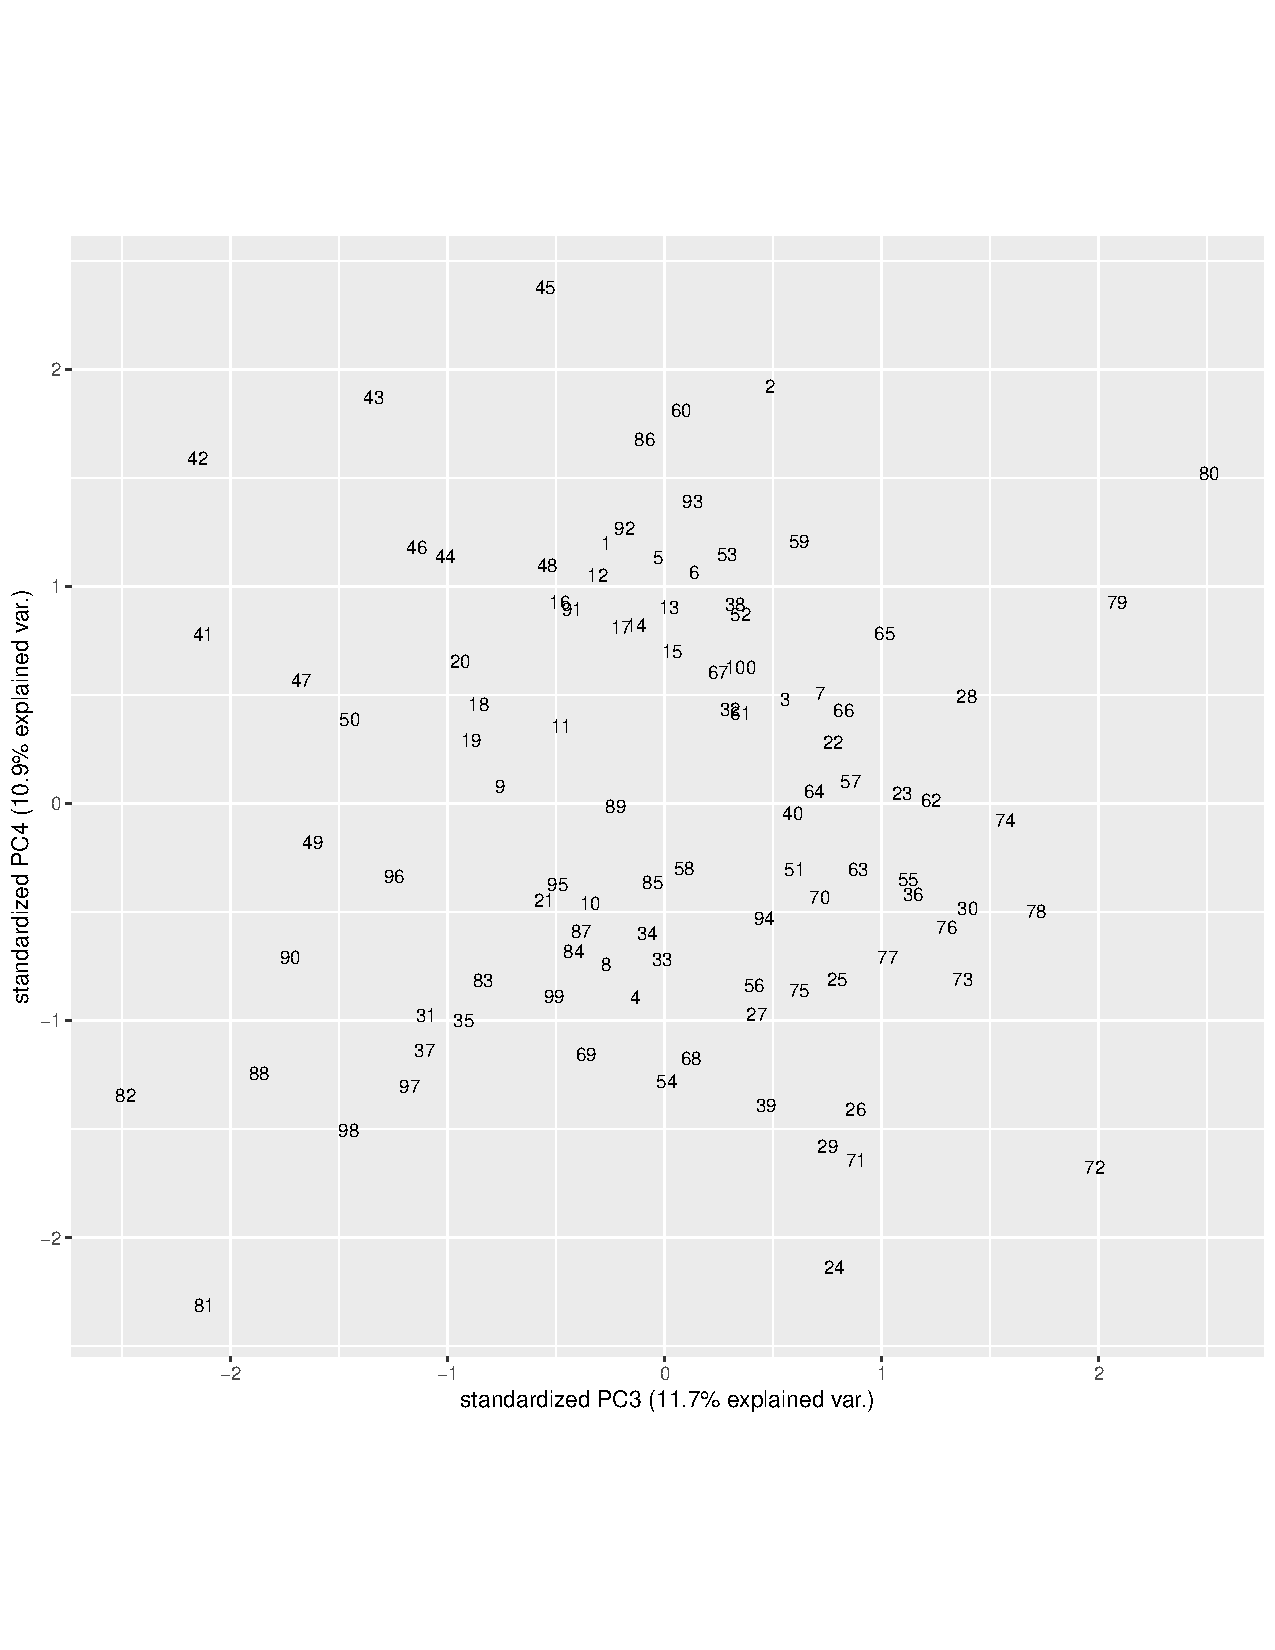
\includegraphics[width=5cm]{billeder/pca2.pdf} }}%
	\caption{Left: A plot of the first two principle components of the data. Right: A plot of the third and fourth principle component. The numbers from 1 to 100 illustrate the date projected onto the principle components}%
	\label{fig:example}%
\end{figure}

\noindent In order to perform a series of ANOVAs, the variables need to be normally distributed and independent. This assumption is shown for a couple of variables below.

\begin{figure}[H]
	\centering
	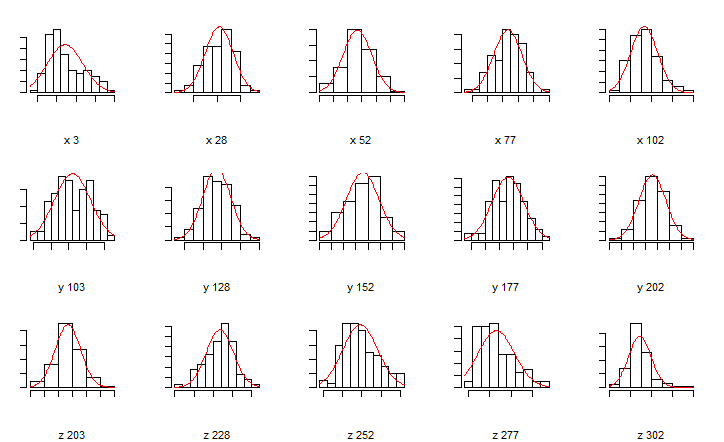
\includegraphics[width=0.7\linewidth]{billeder/normalAF}
	\caption{Histograms for some of the data. In this case a historgram of: x1, x26, x50, x75, x100, y1, y26, y50, y75, y100, 1z, z26, z50, z75, z100. The plots show that the variables are normally distributed.}
	\label{fig:normalaf}
\end{figure}

\noindent Here, it is easy to see that the datapoints are normally distributed or pretty close to normally distributed.

\section{Methods}
%\textit{Describe the methods you used and why you decided to use them. Also discuss the assumptions behind the methods. Do not go into detail with theory.}

\subsection*{Models}
Two different models are constructed in order to classify a specific test subject based on the resulting curve of the arm trajectories. Thsese models are a Binary Classification Tree and a K-nearest neighbors classifier.

\subsubsection*{Binary Classification Tree}
One of the machine learning models used for classification is a binary classification tree. A classification tree is constructed by splitting data into subsets. In the case of a binary classification tree each branch is split into two subsets. The splitting is based on Hunt's algorithm, and the best split is the one with the highest purity gain. The splitting ends when the splits no longer add value to the predictions. 

\subsubsection*{K-nearest neighbors}
The second machine learning model used for classification is a K-nearest neighbor classifier. The model is constructed by storing all of the data. When the model predicts, it chooses the K nearest neighbors with euclidean distance as the measure. The model implemented in this project uses majority voting, and if there is a tie between the neighbors the closest neighbor is chosen as the prediction. As for this experiment, the classifier uses $ K=3 $ nearest neighbors based on pilot experiments.

\subsection*{Comparison of models}
To statistically compare the models, a McNemar's test is chosen. The models are compared under the following hypothesis. 

\begin{align*}\label{key}
H_0 : & \hat \theta_1 =  \hat \theta_2 \\
H_1 : & \hat \theta_1 \neq  \hat \theta_2
\end{align*}
Where $ \hat \theta_1 $ and $ \hat \theta_2  $ are the estimated accuracies of the models. The \textbf{n} matrix is calculated as, 
\begin{equation*}\label{key}
\begin{aligned}
n_{11} &=\sum_{i=1}^{n} c_{i}^{A} c_{i}^{B} \qquad= \{ \text{Both classifiers are correct} \} \\
n_{12} &=\sum_{k=1}^{n} c_{i}^{A}\left(1-c_{i}^{B}\right) \quad=\{A \text { is correct, } B \text { is wrong }\} \\
n_{21} &=\sum_{k=1}^{n}\left(1-c_{i}^{A}\right) c_{i}^{B} \quad=\{A \text { is wrong, } B \text { is correct }\} \\
n_{22} &=\sum_{k=1}^{n}\left(1-c_{i}^{A}\right)\left(1-c_{i}^{B}\right)=\{\text { Both classifiers are wrong }\}
\end{aligned}
\end{equation*}
\noindent
The p-value is then calculated using the following expression, 
\begin{equation}\label{key}
p=2 \mathrm{cdf}_{\mathrm{binom}}\left(m=\min \left\{n_{12}, n_{21}\right\} | prop=\frac{1}{2}, N=n_{12}+n_{21}\right)
\end{equation}
\noindent
The interpretation is that the lower p is, the more evidence there is for A being better than B, but this is only to be interpreted along with the confidence interval given by the following expression.

\begin{equation}\label{key}
\begin{aligned}
&\theta_{L}=2 \operatorname{cdf}_{B}^{-1}\left(\frac{\alpha}{2} | \alpha=p, \beta=q\right)-1\\
&\theta_{U}=2 \operatorname{cdf}_{B}^{-1}\left(1-\frac{\alpha}{2} | \alpha=p, \beta=q\right)-1
\end{aligned}
\end{equation}
\noindent
If zero is not observed in the interval given by, $ [\theta_{L},\theta_{U}] $ and the p-value is significant, then model A is better than model B \cite{mlbog}.

\subsection*{Test-statistics}
To test whether there is a significant effect of experiment on the resulting curve an analysis of variance is used as a statistical test. 

\subsubsection*{Analysis of Variance: ANOVA}
ANOVA is used when all the explanatory variables are factors. In the case of this experiment there are four explanatory variables, namely the person, repetition, experiment and whether it is an x,y or z coordinate. The response variable is the position, i.e. the resulting curve. A two-way Anova with experiment and person as explanatory variables are conducted for each of the x1 coordinates, y2 coordinates, z3 coordinates etc. as response variables. This leads to 300 separate Anovas and yields 300 different p-values. The null hypothesis is that all the resulting curves in each experiment comes from the same population and therefore, there is no difference in the means of the resulting curves. The reason why several Anovas is chosen rather than a set of t-test is due to the fact that Anova minimizes the type I error. The p values obtained are then adjusted by the Benjmain Hochberg method. On a level of significance at $ \alpha = 0.05 $, it would be expected that at least 5\% of the \textit{p}-values are below $ \alpha $. \cite{statbog}


\section{Results}
%\textit{Present the results. \\ Tables and figures are good ways of illustrating results.} \\
Using the 3-nearest neighbor and binary classification tree models to classify the person from the curve yielded the following results.

\begin{table}[h]
	\centering
	\begin{tabular}{l r}
		\toprule
		Classification Model       & Accuracy  \\ \midrule
		Baseline                   & 0.12      \\
		3-Nearest neighbor         & 0.64      \\ 
		Binary classification tree & 0.47      \\ \bottomrule
	\end{tabular}
\caption{The accuracies of the three models}
\label{accuracies}
\end{table}

\noindent To test if this difference between accuracies is significant, and if the models are significantly different, McNemar's test has been performed. The result of this test is shown below.

\[n = \begin{bmatrix} n_{11} & n_{12} \\ n_{21} & n_{22} \end{bmatrix} = \begin{bmatrix} \text{Both classifiers are correct} & \text{One classifier is correct} \\ \text{The other classifier is correct} & \text{Both classifiers are wrong} \end{bmatrix} = \begin{bmatrix} 38 & 26 \\ 9 & 27 \end{bmatrix}\] 

\begin{table}[H]
	\centering
	\begin{tabular}{l r}
		\toprule
		Measure        & Value                          \\ \midrule

		\textbf{KNN \& Decision tree} &                 \\		
		$\hat{\theta}$ & 0.17                           \\ 
		p-value        & 0.00599                        \\ 
		CI             & $0.0585 \leq 0.170 \leq 0.279$ \\ \midrule

		\textbf{KNN \& Baseline} &                      \\		
		$\hat{\theta}$ & 0.52                           \\ 
		p-value        & $2.260 \cdot 10^{-13}$      \\ 
		CI             & $0.407 \leq 0.520 \leq 0.624$ \\ \midrule
		
		\textbf{Decision tree \& Baseline} &            \\
		$\hat{\theta}$ & 0.35                           \\ 
		p-value        & $6.867 \cdot 10^{-7}$       \\ 
		CI             & $0.226 \leq 0.350 \leq 0.468$ \\ \bottomrule
		
	\end{tabular}
\caption{Statistics for difference in mutual accuracies between KNN, decision tree and baseline.}
\label{measuresKNNDT}
\end{table}

\noindent Using ANOVA, the following results have been gathered for investigating whether the experiment has a significant effect on the resulting curve.

\begin{figure}[H]
	\centering
	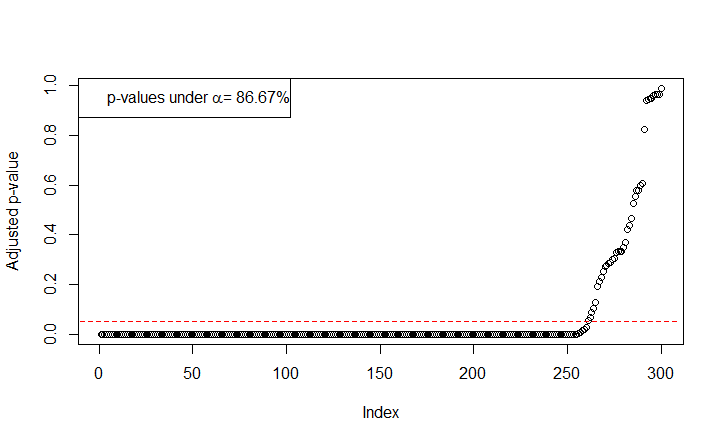
\includegraphics[width=0.7\linewidth]{billeder/pvals_res.png}
	\caption{A plot of the adjusted \textit{p}-values. The plot contains 300 different p-values and has a threshold at the level of significance, $ \alpha = 0.05 $. The legend shows that 86.67 \% p-values  are below the level of significance, which in turn makes experiment statistically significant for the resulting curve. }
	\label{fig:pvalsres}
\end{figure}




%\begin{figure}[H]
%	\centering
%	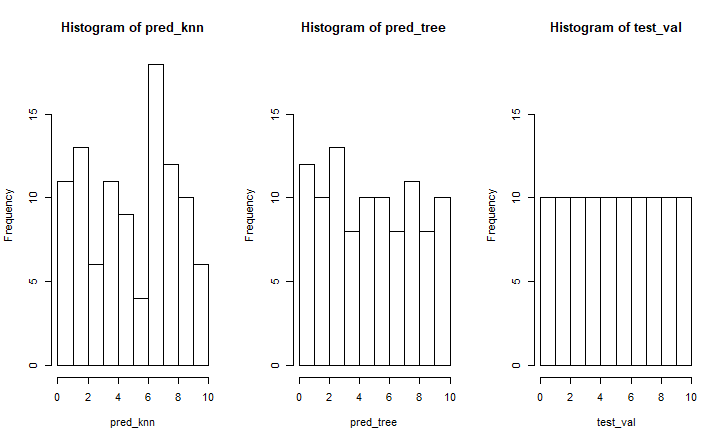
\includegraphics[width=0.7\linewidth]{billeder/PredHist.png}
%	\caption{}
%	\label{fig:predhist}
%\end{figure}

\section{Discussion}
%\textit{What do your results show? \\ Discuss your results. How reliable are they?} \\
From \ref{accuracies} in the results, it is clear that is it somewhat possible to predict the person that performed a movement based only on that person's movement curve. The baseline, which simply samples a number from 1 to 10 for the prediction, got an accuracy of 0.12, which is close to what is expected when dealing with 10 classes. Performing three McNemar's tests to test the differences between accuracies between KNN and the decision tree, KNN and baseline as well as decision tree and baseline, the results of which are shown in \ref{measuresKNNDT}, it is clear that both of the models are significantly better than baseline, since both of these p-values are under 0.05. Meanwhile, it is also clear that the KNN model is better than the decision tree with a p-value of 0.00599. The difference between the values of the accuracies is around $0.0585 \leq 0.170 \leq 0.279$. As such, it is evident that the KNN model would be a better machine learning model to apply to this problem. Furthermore, it would be reasonable to expect that a more complex model like a neural network would get a much higher accuracy, but this is left as future work.
%\\\\
%For the test of whether experiment has a significant effect on the resulting curve, ANOVA has been performed which results in the third table of the results. Here, it is very obvious that every explanatory variable is extremely significant, as every p-value is $<2.200 \cdot 10^{-16}$. This would imply that position, repetition, person and experiment has an influence on how the curve ends up looking. This could make sense since position is directly correlated with the curve and people have different movement patterns, which was also evident from the other question of this paper. Since the different experiments have obstacles of varying heights and therefore results in different curves. The significance of the repetition on effect of the curve seems slightly more mysterious, but this can be explained by the fact that no one is able to move in the exact same way 10 times in a row, so the variances in every repetition is statistically significant for the curve. From figure \ref{fig:rplot} it is also seen that each curve in the repetition varies a notable amount, which could explain why it is statistically significant variable for the resulting curve. 
\\\\
For the test of whether experiment has a significant effect on the resulting curve, ANOVA has been performed 300 times, which results in the plot seen in figure \ref{fig:pvalsres}. From the results 86.67 \% of the p-values are below the desired level of significance. Here it is very obvious that experiment is indeed significant. This would imply that experiment has a great effect of how the curve ends up looking.
\begin{figure}[H]
	\centering
	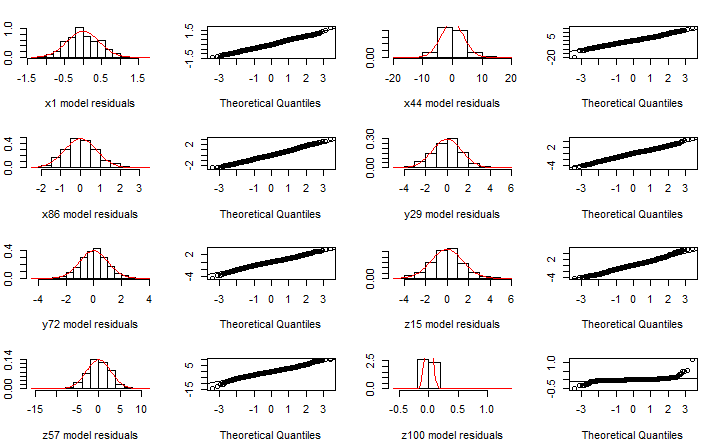
\includegraphics[width=0.7\linewidth]{billeder/StadigNormalfordeltAF.png}
	\caption{This figure shows some of the residuals from the ANOVA models constructed. Furthermore, it is seen that most the residuals from the constructed models are normally distributed. }
	\label{fig:stadignormalfordeltaf}
\end{figure}
 Figure \ref{fig:stadignormalfordeltaf} represents some of the constructed model residuals. It is revealed that most of the residuals from the constructed models are normally distributed, which makes the analysis of variance valid. Some of the residuals are not normally distributed, an example is z100, seen in figure \ref{fig:stadignormalfordeltaf}. On the other hand $ 86.67 $ \% of the p-values are below $ 0.05 $ and only 5\% of the p-values need to be below $ \alpha $ in order for experiment to be significant for the resulting curve. Thus, if some of the p-values are removed one could argument that experiment still would be significant for the resulting curve. The finding also makes sense, since each experiment has different heights in which the test participants have to move the cylindrical object. 


\section{Conclusion}
%\textit{What are your conclusions? The conclusion should be connected to the aim of the report in the introduction. \\ Highlight important results \\ If you have found interesting problems/aspects that you haven’t carried out, you can specify them here as ‘future work’.}

In this paper, two important questions have been investigated. The first question is whether it is possible to use a 3-nearest neighbor and binary decision tree machine learning model to classify the person performing an experiment based on the a given movement curve, and which model is best at performing this classification. Based on the accuracies of the KNN and decision tree models in comparison to baseline, it is pretty safe to say that it is possible to use a machine learning model to predict the person based on the movement curve. Especially more complex machine learning models could be very successful for this prediction task, but actually implementing these more complicated models has been left for future work. For comparing the two models to each other, McNemar's test has been used, which showed that there is a significant difference in the accuracies of the two models and that both models are significantly different from the baseline. As such, if one of the two models produced in this paper should be used to classify the person, the KNN model is recommended.

The second question was if the performed experiment had a significant effect on the resulting movement curve. To investigate this problem, 300 ANOVA have been performed, and it was evident that there is a big significance of person and experiment on the resulting curve. For future papers, it could be interesting to use other test statistics to reinforce this result. From the result of the ANOVAs, it is clear that experiment has an effect on how the curve turns out, which can be thought of as logical, since the experiments vary in obstacle sizes. Therefore, the subject has to use arm movements of varying sizes to move the object over the obstacle, resulting in a vastly different curve.
\newpage
\section{Appendix}
Link to GitHub to see code:
\url{https://github.com/oskarwiese/project02445.git}
	
\bibliographystyle{IEEEbib}
\bibliography{refs}

\end{document}
